\documentclass{article}
\usepackage{hyperref}
\usepackage{float}
\usepackage{graphicx}
\usepackage{xcolor}
\usepackage{siunitx}
\usepackage[margin=1in]{geometry}

\newcommand{\red}[1]{\textcolor{red}{#1}}
\newcommand{\green}[1]{\textcolor{green}{#1}}
\newcommand{\brown}[1]{\textcolor{brown}{#1}}

\begin{titlepage}
    \title{GCRC Hackathon 1}
    \author{Martin Jasinski, Nane Vardanyan, Cynthia Shaheen}
    \date{\today}
\end{titlepage}

\begin{document}
    \maketitle
    
    \section{Background}
    Antisense oligonucleotides (ASOs) are promising therapeutic molecules for targeting disease-associated RNA transcripts, but evaluating their specificity and molecular interactions remains challenging. Conventional bulk assays primarily characterize ASO-RNA interactions at equilibrium, limiting their ability to resolve the dynamic association and dissociation events that govern target engagement. Here, we are developing a single-molecule platform that combines CLiC nanowell confinement with Förster resonance energy transfer (FRET) to characterize ASO-RNA interactions in real time. 
    \begin{figure}[hbtp!]
        \centering
        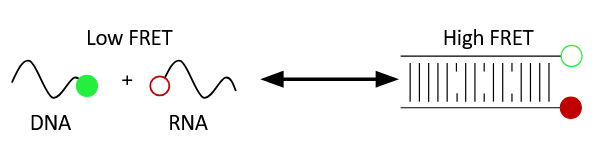
\includegraphics[width=0.8\textwidth]{3MM_aso_diagram.png}
        \label{fig:diagram_aso}
    \end{figure}
    \section{Problem Statement}
    You are provided with a dataset consisting of single-microscopy images of two complementary RNA strands diffusing in nanowells, shown in the graphic in Fig. \ref{fig:diagram_aso}. The RNAs have fluorophores on the $5'$ ends of each RNA and are excited with a \red{$\SI{647}{\nano\meter}$} and \green{$\SI{532}{\nano\meter}$} laser respectfully. The captured images as sequences such that they are labelled with alternating frames in the following pattern:
    \begin{equation}
        V:\{\red{F_1}, \green{F_2}, \brown{F_3}, \red{F_4}, \green{F_5} \dots\}\,
    \end{equation}
    where \red{red} signifies the use of the 647 laser, \green{green} signifies the use of a 532 laser, and \brown{sienna} signifies use of both lasers.

    Your task is simple, analyze the videos and to find the transverse positions $x,y$ of each particle in each frame, and determine colocalized videos. 

    The output of the code should consist of a \textsc{CSV} file that consists of the following parameters:
\begin{table}[htbp]
\centering
\caption{Example: Output \textsc{CSV} structure}
\label{tab:particle_data}
\resizebox{\columnwidth}{!}{\begin{tabular}{|cccccc|}
\hline
\textbf{Particle} & \textbf{Video} & \textbf{$xy_1(t)$} & \textbf{$xy_2(t)$} & \textbf{${I_1(t)}$} & ${I_2(t)}$\\ \hline
P01               & Vid\_1         & [(12.4, 45.2), (12.2, 47.1), \dots]   & [(12.6, 45.8), (10.2, 43.1), \dots]   & [1.23, 3.24, 1.5, \dots]& [1.23, 3.22, 1.0, \dots]                  \\
P02               & Vid\_1         & [(89.1, 12.3), (50.2, 30.1), \dots]   & [(89.0, 12.9), (88.2, 13.1), \dots]   & [3.43, 0.34, 1.21, \dots]& [7.47, 4.56, 6.9, \dots]                   \\
P03               & Vid\_2         & [(34.7, 78.1), (30.2, 77.1), \dots]   & [(35.2, 77.9), (33.2, 78.1), \dots]   & [4.13, 1.55, 1.73, \dots]& [2.67, 5.21, 8.4, \dots]                  \\
\vdots               & \vdots         & \vdots   & \vdots   & \vdots& \vdots                  \\ \hline
\end{tabular}}
\end{table}
%     \begin{table}[htbp]
% \centering
% \caption{Example: Output \textsc{CSV} structure}
% \label{tab:particle_data}
% \begin{tabular}{|cccccc|}
% \hline
% \textbf{Particle} & \textbf{Video} & \textbf{$xy_1(t)$} & \textbf{$xy_2(t)$} & \textbf{${I_1(t)}$} & ${I_2(t)}$\\ \hline
% P01               & Vid\_1         & [(12.4, 45.2), (12.2, 47.1), \dots]   & [(12.6, 45.8), (10.2, 43.1), \dots]   & [1.23, 3.24, 1.5, \dots]& [1.23, 3.22, 1.0, \dots]                  \\
% P02               & Vid\_1         & [(89.1, 12.3), (50.2, 30.1), \dots]   & [(89.0, 12.9), (88.2, 13.1), \dots]   & [3.43, 0.34, 1.21, \dots]& [7.47, 4.56, 6.9, \dots]                   \\
% P03               & Vid\_2         & [(34.7, 78.1), (30.2, 77.1), \dots]   & [(35.2, 77.9), (33.2, 78.1), \dots]   & [4.13, 1.55, 1.73, \dots]& [2.67, 5.21, 8.4, \dots]                  \\
% \vdots               & \vdots         & \vdots   & \vdots   & \vdots& \vdots                  \\ \hline
% \end{tabular}
% \end{table}

\end{document}